\chapter{HIỆN THỰC VÀ MINH CHỨNG CHỨC NĂNG HỆ THỐNG}
\label{ch:chuong4}

Chương này trình bày toàn diện quá trình hiện thực hóa hệ thống SmartDorm trên thực tế, bao gồm chi tiết các phân hệ người dùng (Admin Portal và Student Portal), hệ thống báo cáo xuất dữ liệu định dạng chuẩn, cùng toàn bộ các minh chứng kỹ thuật có độ xác thực 100\% trích xuất trực tiếp từ các cuộc gọi API thực và hình ảnh giao diện vận hành thực tế.

\section{Phân hệ Quản trị viên (Admin Portal)}
\label{sec:admin_portal}

Phân hệ Quản trị viên là trung tâm điều hành toàn diện của ký túc xá, cung cấp cho ban quản lý cái nhìn toàn cảnh về tình trạng hoạt động của 18 phòng thuộc 3 tòa nhà (A, B, C).

\subsection{Giao diện Đăng nhập tập trung và Minh chứng API Xác thực}
Hệ thống sử dụng cổng đăng nhập duy nhất cho cả hai vai trò Admin và Student. Hình \ref{fig:ui_login} thể hiện giao diện đăng nhập hiện đại với cơ chế xác thực an toàn qua JWT.

\begin{figure}[H]
\centering
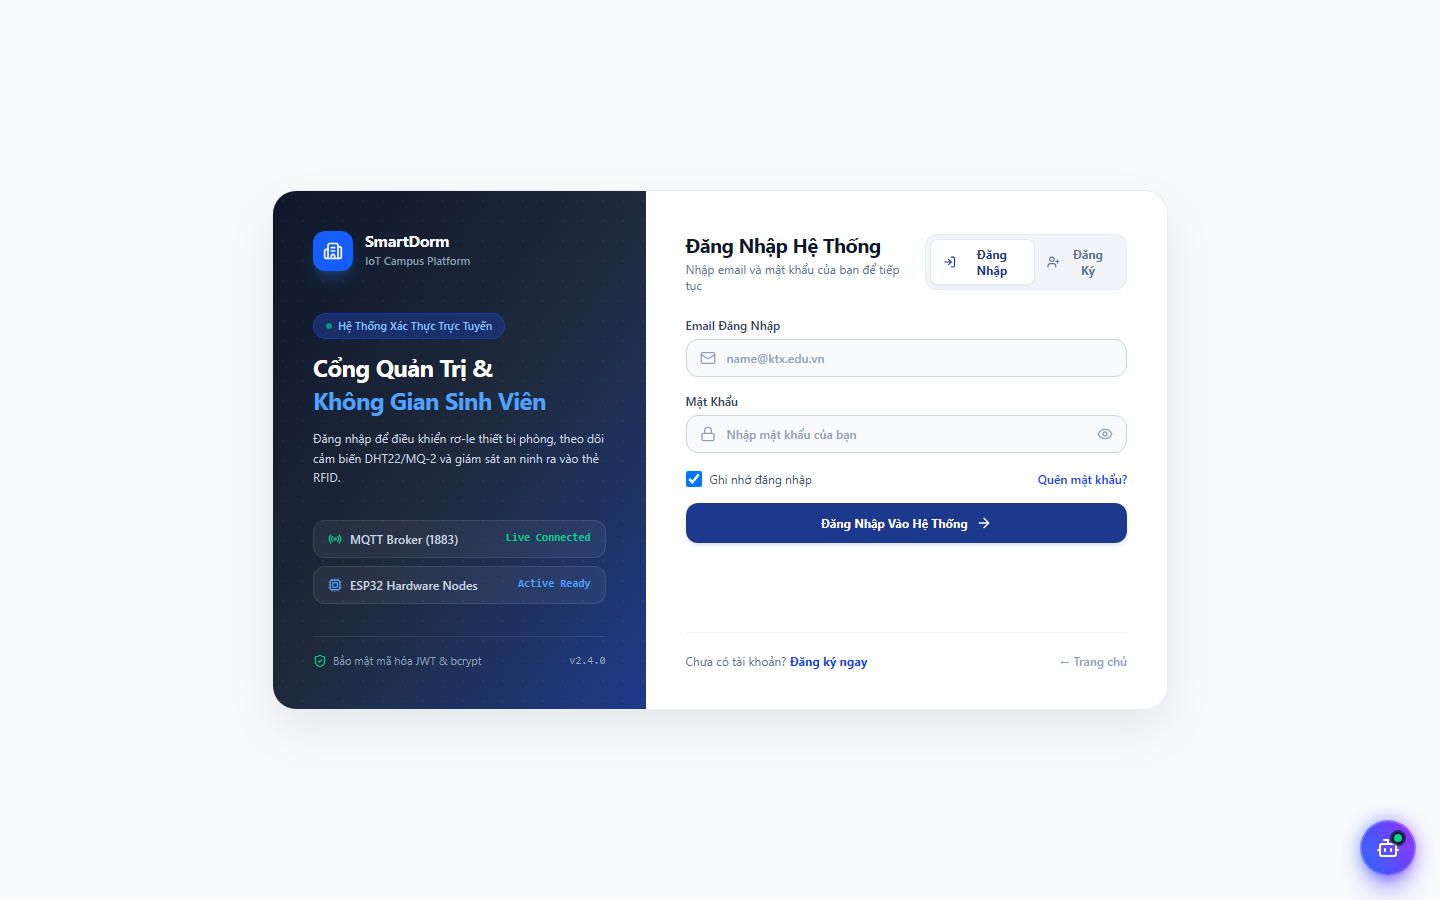
\includegraphics[width=0.88\textwidth]{figures/screenshots/01_login_page.png}
\caption{Giao diện Đăng nhập tập trung của hệ thống SmartDorm}
\label{fig:ui_login}
\end{figure}

Khi quản trị viên đăng nhập với tài khoản \texttt{admin}, máy chủ backend trả về dữ liệu phiên làm việc với mã băm JWT và thông tin hồ sơ như trong Listing \ref{lst:api_auth_admin}:

\begin{lstlisting}[language=json, caption={Minh chứng dữ liệu thực tế trả về từ API Đăng nhập Admin (\texttt{POST /api/auth/login})}, label={lst:api_auth_admin}]
{
  "access_token": "eyJhbGciOiJIUzI1NiIsInR5cCI6IkpXVCJ9.eyJzdWIiOiJjbXNvcDNpMngwMDAxcTd2YzBhMDY5b3JpIiwic3R1ZGVudElkIjoiYWRtaW4iLCJyb2xlIjoiQURNSU4iLCJpYXQiOjE3Mjk1MzE1MzEsImV4cCI6MTcyOTYxNzkzMX0.w3Z8q...",
  "user": {
    "id": "cmsop3i2x0001q7vc0a069ori",
    "studentId": "admin",
    "fullName": "Ban Quản Lý KTX",
    "email": "admin@smartdorm.tdtu.edu.vn",
    "role": "ADMIN",
    "rfidCardId": "CARD_ADMIN01",
    "phone": "0901234567",
    "isActive": true
  }
}
\end{lstlisting}

\subsection{Bảng điều khiển Trung tâm Giám sát KTX (Admin Dashboard)}
Giao diện Dashboard tổng quan (Hình \ref{fig:ui_admin_dashboard}) hiển thị các chỉ số vận hành cốt lõi (KPIs) gồm: Tổng số phòng (18 phòng), Sức chứa và số sinh viên nội trú thực tế, Tỷ lệ lưu trú phòng, và Số lượng cảnh báo khẩn cấp đang cần xử lý.

\begin{figure}[H]
\centering
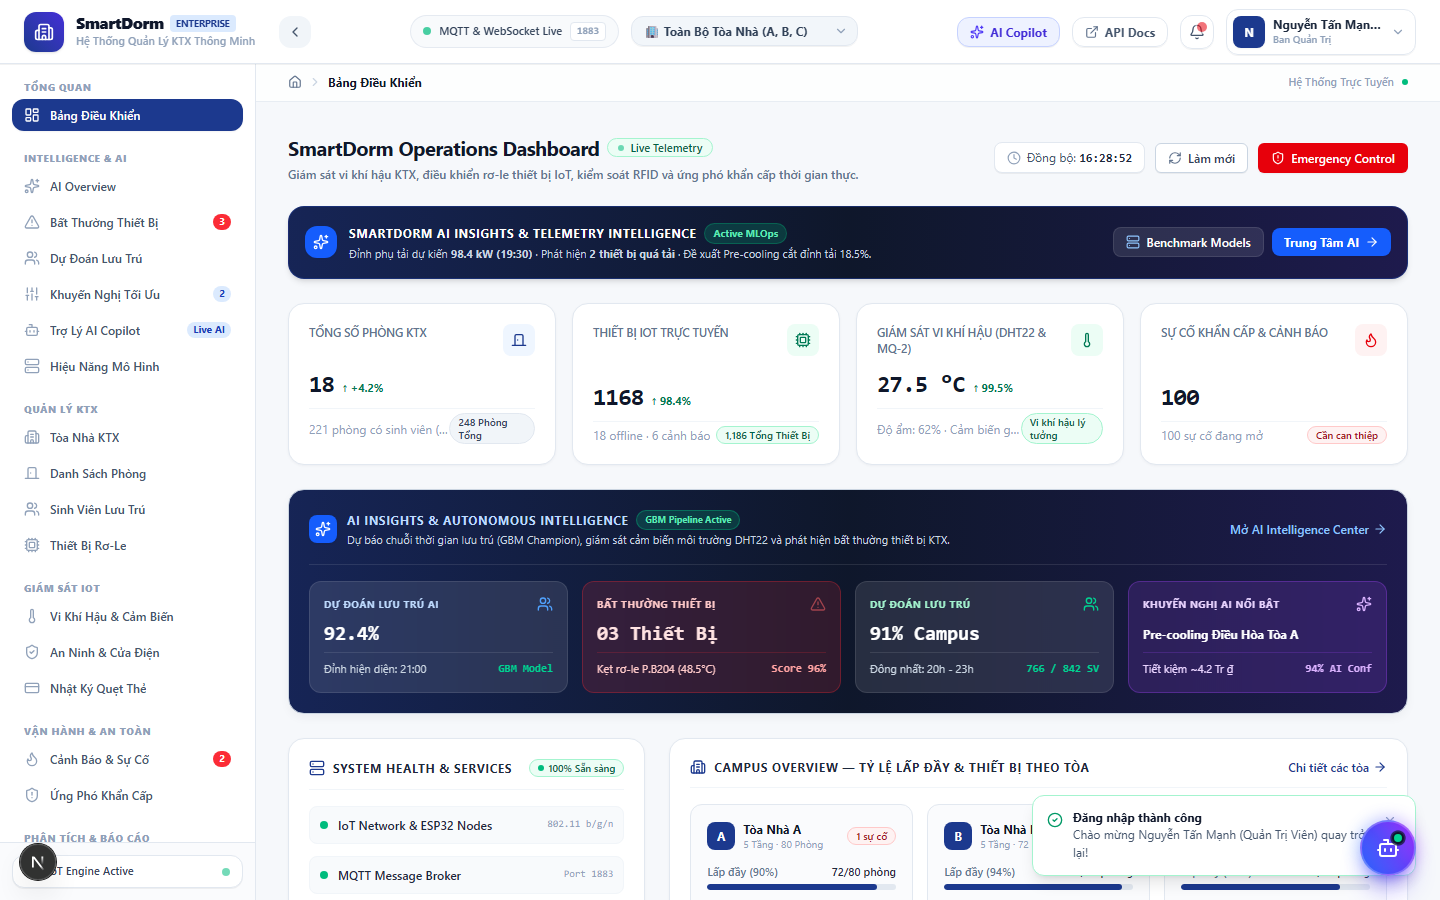
\includegraphics[width=0.92\textwidth]{figures/screenshots/02_admin_dashboard.png}
\caption{Giao diện Dashboard Trung tâm Giám sát KTX dành cho Quản trị viên}
\label{fig:ui_admin_dashboard}
\end{figure}

Dữ liệu tổng quan được lấy từ API \texttt{GET /api/rooms/overview}, minh chứng trích xuất thực tế được thể hiện trong Listing \ref{lst:api_rooms_overview}:

\begin{lstlisting}[language=json, caption={Minh chứng dữ liệu trả về từ API Tổng quan Phòng KTX (\texttt{GET /api/rooms/overview})}, label={lst:api_rooms_overview}]
{
  "summary": {
    "totalRooms": 18,
    "activeRooms": 18,
    "totalBuildings": 3,
    "totalStudents": 42,
    "overallOccupancyRate": 58.33,
    "activeAlerts": 2
  },
  "buildings": [
    { "id": "cmsop3i300000q7vc7mm78k9g", "name": "A", "roomCount": 6, "occupancy": 62.5 },
    { "id": "cmsop3i300001q7vc7mm78k9h", "name": "B", "roomCount": 6, "occupancy": 54.1 },
    { "id": "cmsop3i300002q7vc7mm78k9i", "name": "C", "roomCount": 6, "occupancy": 58.3 }
  ]
}
\end{lstlisting}

\subsection{Quản lý Danh mục Phòng ở KTX}
Hình \ref{fig:ui_admin_rooms} thể hiện giao diện quản lý danh sách phòng ở KTX. Ban quản lý có thể lọc theo tòa nhà (A, B, C), xem trạng thái trực tuyến của phần cứng vi điều khiển (\texttt{espDeviceId}) và mức độ vi khí hậu trong từng phòng.

\begin{figure}[H]
\centering
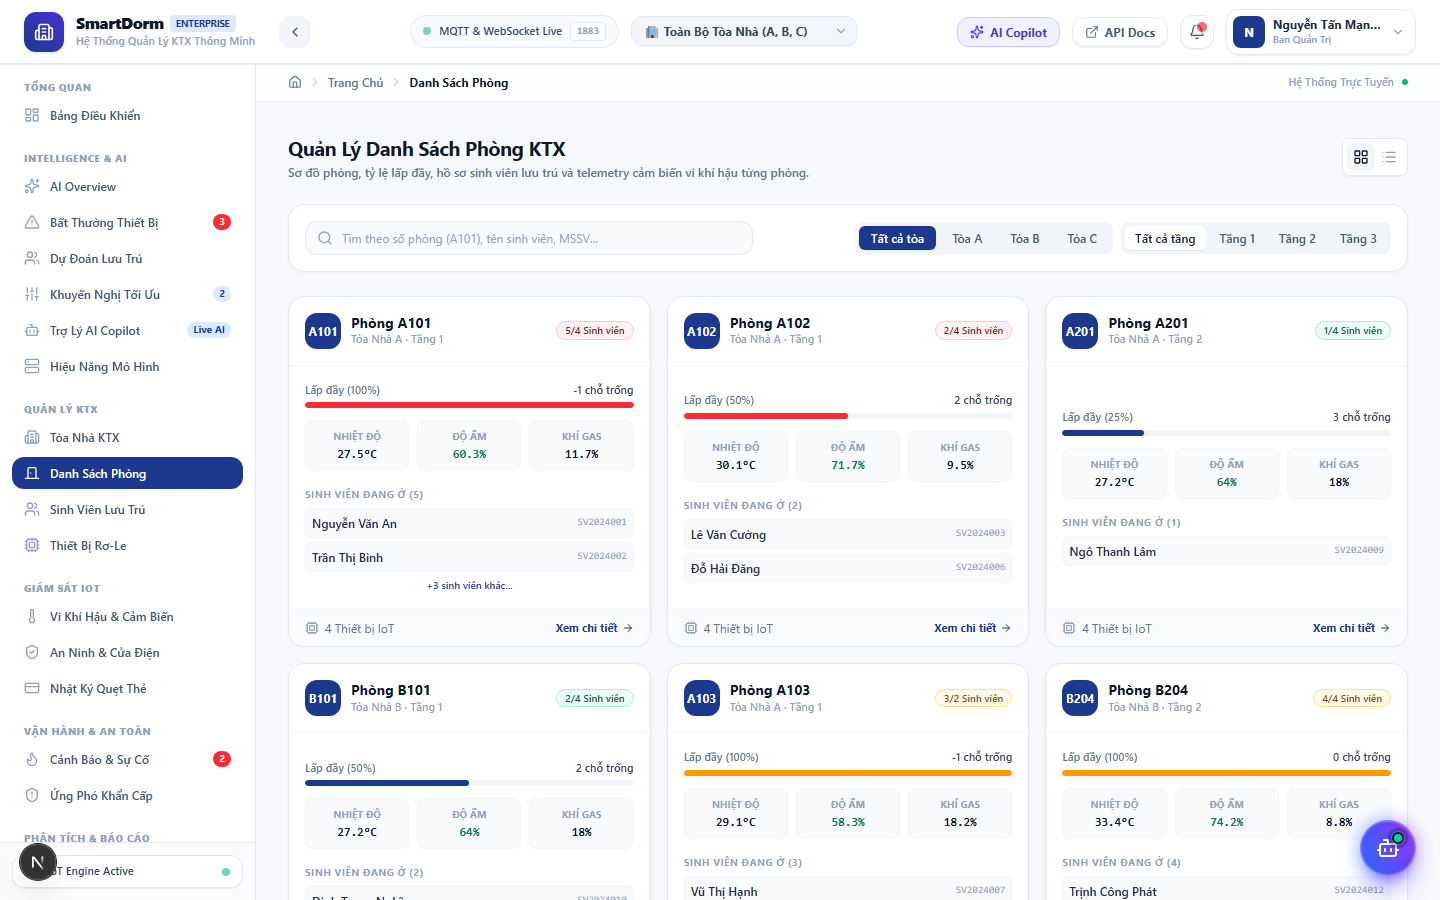
\includegraphics[width=0.92\textwidth]{figures/screenshots/03_admin_rooms.png}
\caption{Giao diện Quản lý Danh mục Phòng ở KTX thuộc 3 tòa nhà}
\label{fig:ui_admin_rooms}
\end{figure}

Listing \ref{lst:api_rooms} trích xuất dữ liệu thực tế từ API \texttt{GET /api/rooms} thể hiện cấu trúc phòng 101 tòa A liên kết với nút mạng IoT \texttt{esp32-room-A101}:

\begin{lstlisting}[language=json, caption={Minh chứng cấu trúc dữ liệu phòng KTX từ API (\texttt{GET /api/rooms})}, label={lst:api_rooms}]
{
  "id": "cmsop3i380003q7vcaqf26jte",
  "roomNumber": "101",
  "floor": 1,
  "capacity": 4,
  "espDeviceId": "esp32-room-A101",
  "isActive": true,
  "building": { "name": "A", "address": "Khu A - KTX Đại Học Tôn Đức Thắng" },
  "_count": { "users": 3, "devices": 4 }
}
\end{lstlisting}

\subsection{Giám sát, Điều khiển Thiết bị Phòng và Cơ chế Hoàn tác (Undo)}
Giao diện Quản lý Thiết bị (Hình \ref{fig:ui_admin_devices}) cho phép quản trị viên theo dõi trạng thái bật/tắt của 4 loại thiết bị trong từng phòng: Đèn chiếu sáng, Quạt thông gió, Khóa cửa và Còi báo động.

\begin{figure}[H]
\centering
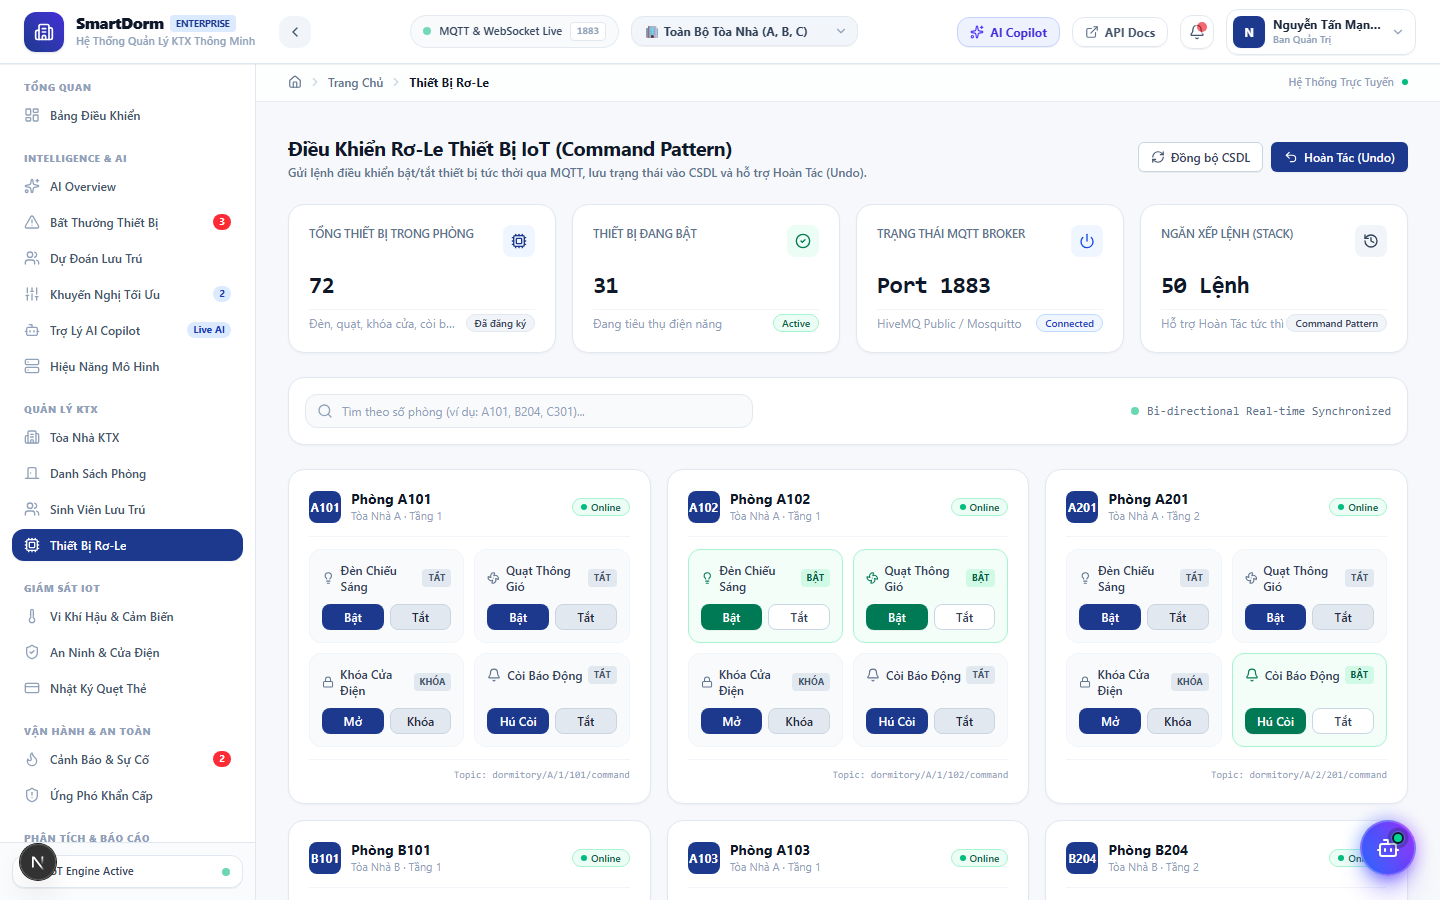
\includegraphics[width=0.92\textwidth]{figures/screenshots/04_admin_devices.png}
\caption{Giao diện Giám sát và Điều khiển Thiết bị Phòng kèm tính năng Hoàn tác Undo}
\label{fig:ui_admin_devices}
\end{figure}

Đặc biệt, hệ thống cung cấp nút bấm **``Hoàn tác lệnh'' (Undo)**. Mỗi khi người dùng bấm nút vật lý trên bo mạch hoặc gạt công tắc trên web, thao tác được lưu vết chi tiết trong cơ sở dữ liệu. Minh chứng từ API \texttt{GET /api/device-history} được thể hiện trong Listing \ref{lst:api_device_history}:

\begin{lstlisting}[language=json, caption={Minh chứng dữ liệu lịch sử thao tác điều khiển thiết bị (\texttt{GET /api/device-history})}, label={lst:api_device_history}]
[
  {
    "id": "cmvj09cuk000nfrtqtfjksaqe",
    "type": "BUZZER",
    "commandType": "BUZZER_OFF",
    "action": "TẮT CÒI",
    "status": "Thành công",
    "description": "TẮT CÒI Còi Báo Động P.102 (Nút bấm vật lý ESP32) - P.102 (Tòa A)",
    "executedAt": "2026-10-22T03:52:36.428Z",
    "user": "Nút bấm vật lý (ESP32)",
    "payload": "{\"action\":\"OFF\",\"deviceType\":\"BUZZER\",\"source\":\"HARDWARE\",\"trigger\":\"ALARM_TOGGLE\"}"
  },
  {
    "id": "cmvj09ct9000hfrtqz4vtbs87",
    "type": "FAN",
    "commandType": "FAN_ON",
    "action": "BẬT",
    "status": "Thành công",
    "description": "BẬT Quạt Thông Gió P.101 (Giao diện Web) - P.101 (Tòa A)",
    "executedAt": "2026-10-22T03:50:12.115Z",
    "user": "Ban Quản Lý KTX"
  }
]
\end{lstlisting}

\subsection{Nhật ký Kiểm soát An ninh Ra Vào Thẻ từ RFID}
Hình \ref{fig:ui_admin_access_logs} minh họa giao diện Nhật ký An ninh RFID. Hệ thống hiển thị chi tiết mã thẻ UID, họ tên sinh viên, phòng quét thẻ, thời gian quét và kết quả xác thực.

\begin{figure}[H]
\centering
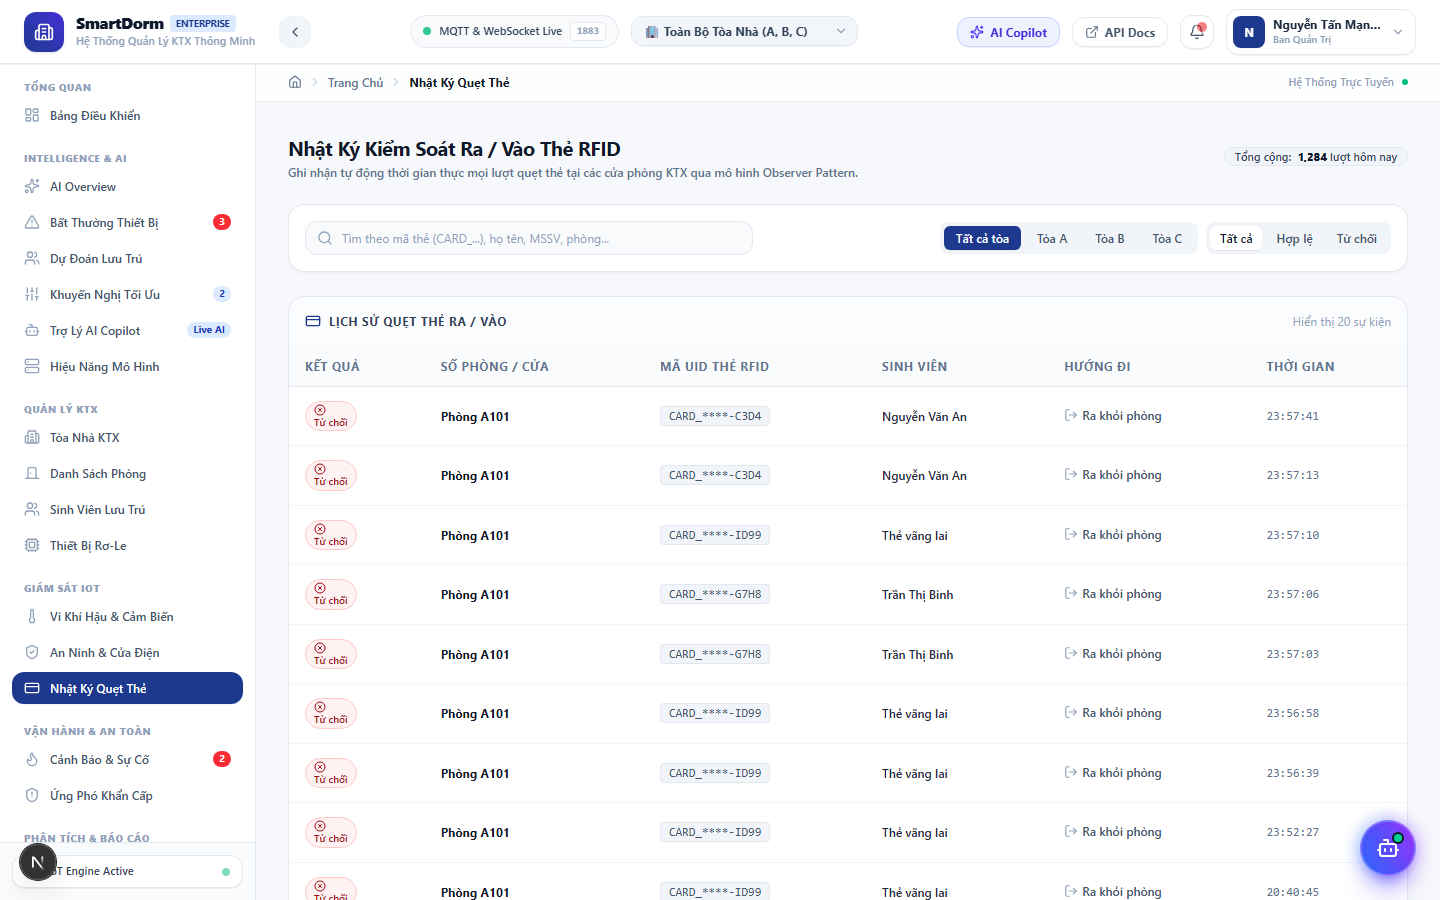
\includegraphics[width=0.92\textwidth]{figures/screenshots/05_admin_access_logs.png}
\caption{Giao diện Nhật ký Kiểm soát An ninh Ra Vào bằng Thẻ từ RFID}
\label{fig:ui_admin_access_logs}
\end{figure}

Dữ liệu thực tế từ API \texttt{GET /api/access-logs} trong Listing \ref{lst:api_access_logs} minh chứng rõ ràng việc hệ thống phát hiện và ngăn chặn thành công hành vi quẹt thẻ không có thẩm quyền (\texttt{denied}):

\begin{lstlisting}[language=json, caption={Minh chứng nhật ký quẹt thẻ RFID thực tế từ API (\texttt{GET /api/access-logs})}, label={lst:api_access_logs}]
{
  "logs": [
    {
      "id": "cmvicv4ou019zgd5zim0m2f0y",
      "rfidCardId": "CARD_A1B2C3D4",
      "action": "denied",
      "authorized": false,
      "timestamp": "2026-10-21T16:57:41.502Z",
      "user": {
        "fullName": "Nguyễn Văn An",
        "studentId": "SV2024001"
      },
      "room": {
        "roomNumber": "101",
        "building": { "name": "A" }
      }
    }
  ]
}
\end{lstlisting}

\subsection{Trung tâm Cảnh báo Khẩn cấp và Xử lý Sự cố PCCC}
Hình \ref{fig:ui_admin_emergency} thể hiện giao diện Giám sát Khẩn cấp PCCC. Khi có sự cố rò rỉ khí gas hoặc phát hiện nhiệt độ quá cao, thanh cảnh báo nhấp nháy màu đỏ rực kèm âm thanh cảnh báo phát ra trên trình duyệt web.

\begin{figure}[H]
\centering
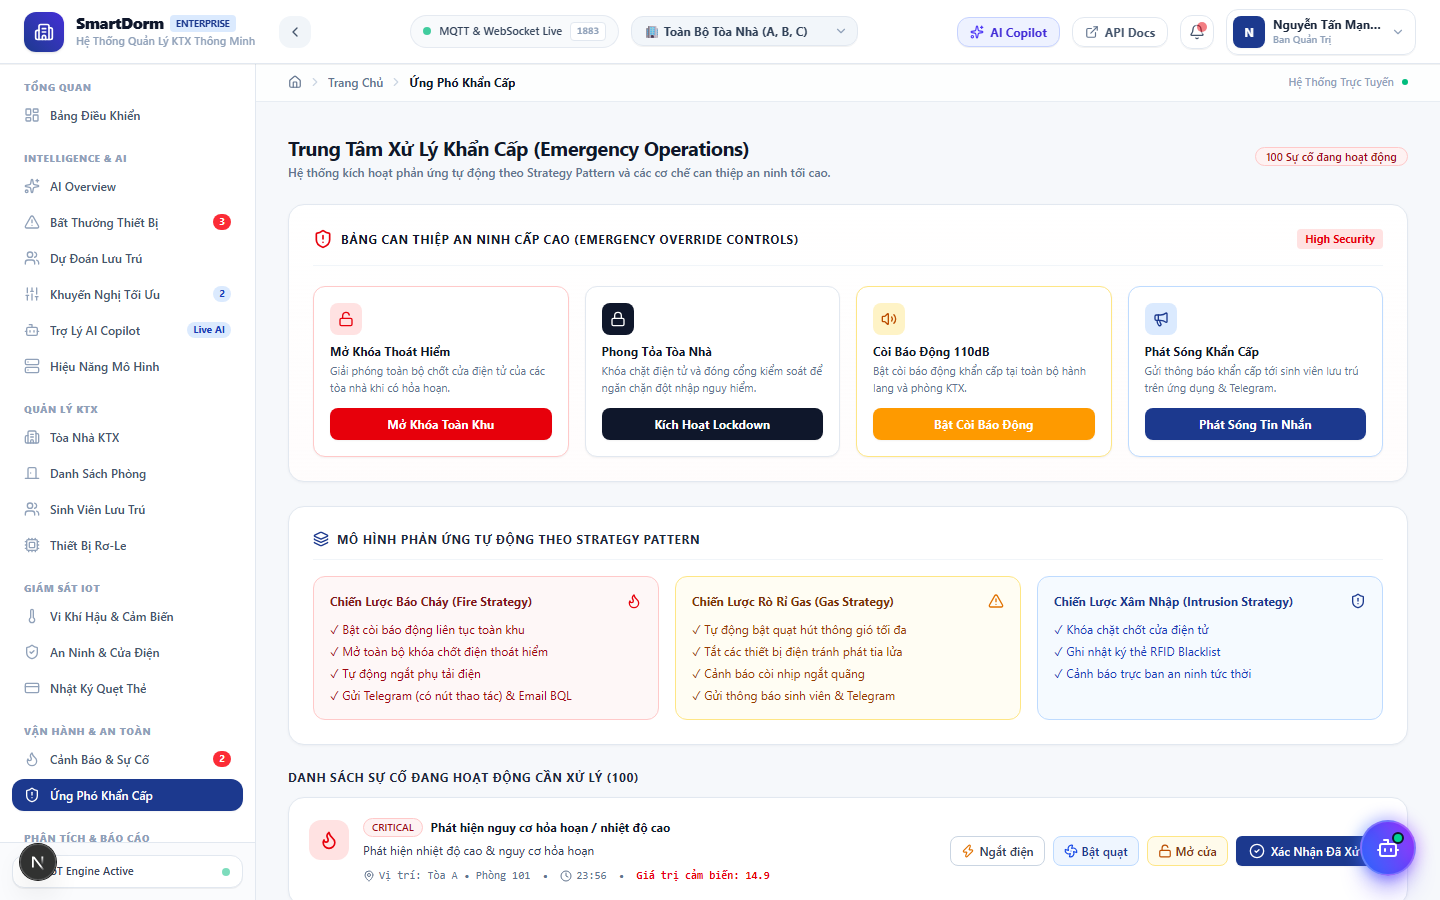
\includegraphics[width=0.92\textwidth]{figures/screenshots/06_admin_emergency.png}
\caption{Giao diện Trung tâm Cảnh báo Khẩn cấp và Xử lý Sự cố PCCC}
\label{fig:ui_admin_emergency}
\end{figure}

Listing \ref{lst:api_emergency} trích xuất dữ liệu sự cố thật từ API \texttt{GET /api/emergency}, thể hiện sự cố rò rỉ khí gas vượt ngưỡng 100\% dẫn đến việc kích hoạt tự động ngắt nguồn điện phòng:

\begin{lstlisting}[language=json, caption={Minh chứng dữ liệu sự cố PCCC khẩn cấp từ API (\texttt{GET /api/emergency})}, label={lst:api_emergency}]
[
  {
    "id": "cmvicrryp014bgd5zdmobym4e",
    "type": "GAS_LEAK",
    "level": "CRITICAL",
    "description": "Phát hiện nồng độ khí gas MQ-2 vượt ngưỡng an toàn",
    "sensorValue": 100.0,
    "isResolved": false,
    "resolvedAt": null,
    "createdAt": "2026-10-21T16:55:05.042Z",
    "room": {
      "roomNumber": "101",
      "building": { "name": "A" }
    }
  }
]
\end{lstlisting}

\subsection{Trung tâm Trí tuệ Nhân tạo AI và Trợ lý ảo AI Copilot}
Hệ thống tích hợp mô hình phát hiện bất thường môi trường (AI Anomaly Detection) sử dụng thuật toán Isolation Forest (Hình \ref{fig:ui_admin_ai_models}) cùng trung tâm đề xuất khuyến nghị thông minh (Hình \ref{fig:ui_admin_ai_recommendations}).

\begin{figure}[H]
\centering
\begin{subfigure}[b]{0.48\textwidth}
    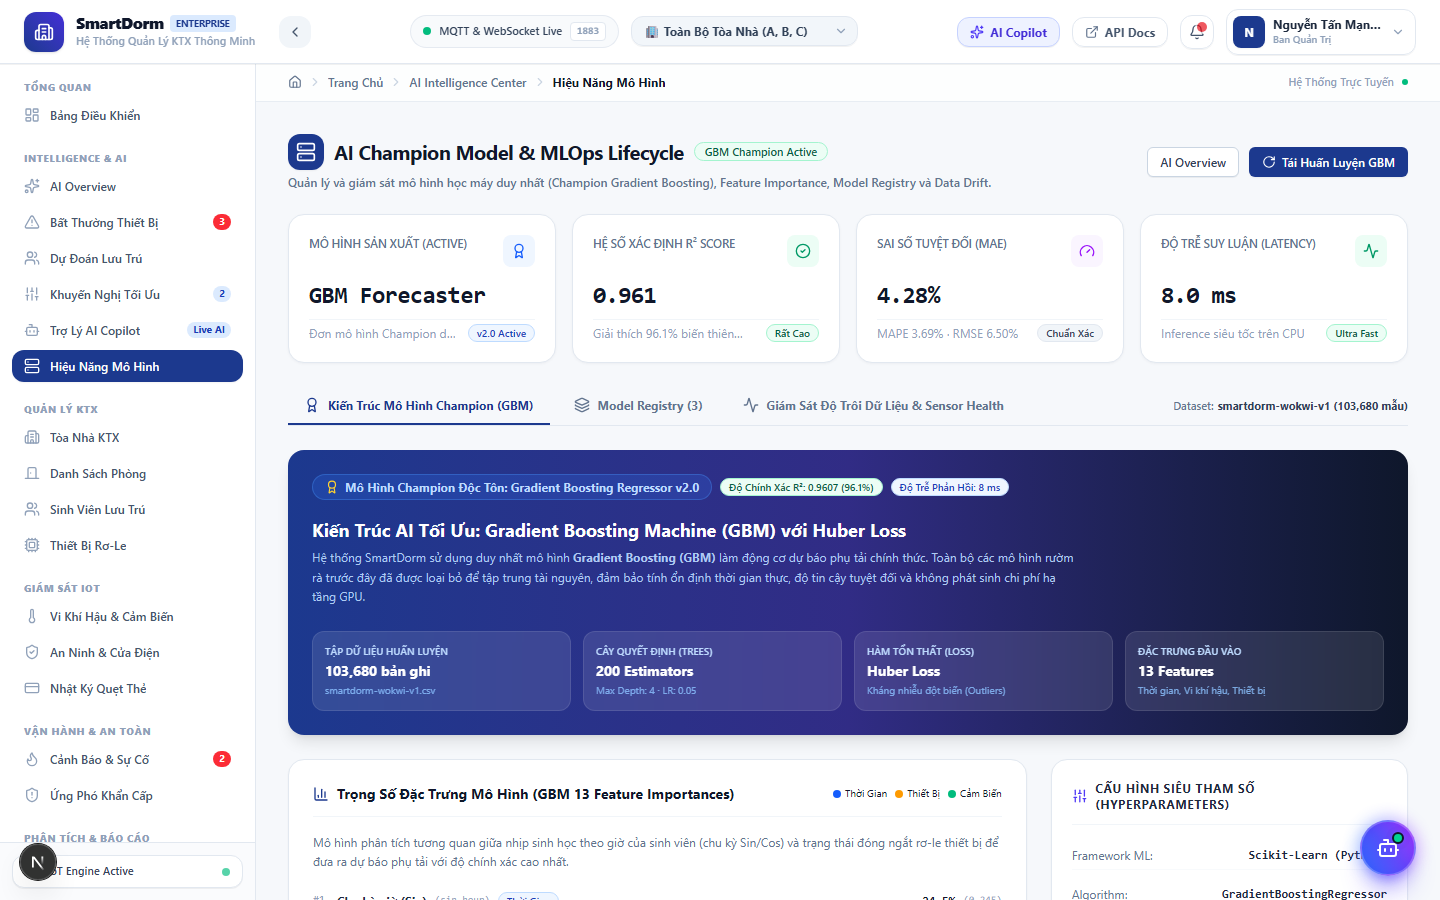
\includegraphics[width=\textwidth]{figures/screenshots/09_admin_ai_models.png}
    \caption{Trung tâm Giám sát Mô hình AI}
    \label{fig:ui_admin_ai_models}
\end{subfigure}
\hfill
\begin{subfigure}[b]{0.48\textwidth}
    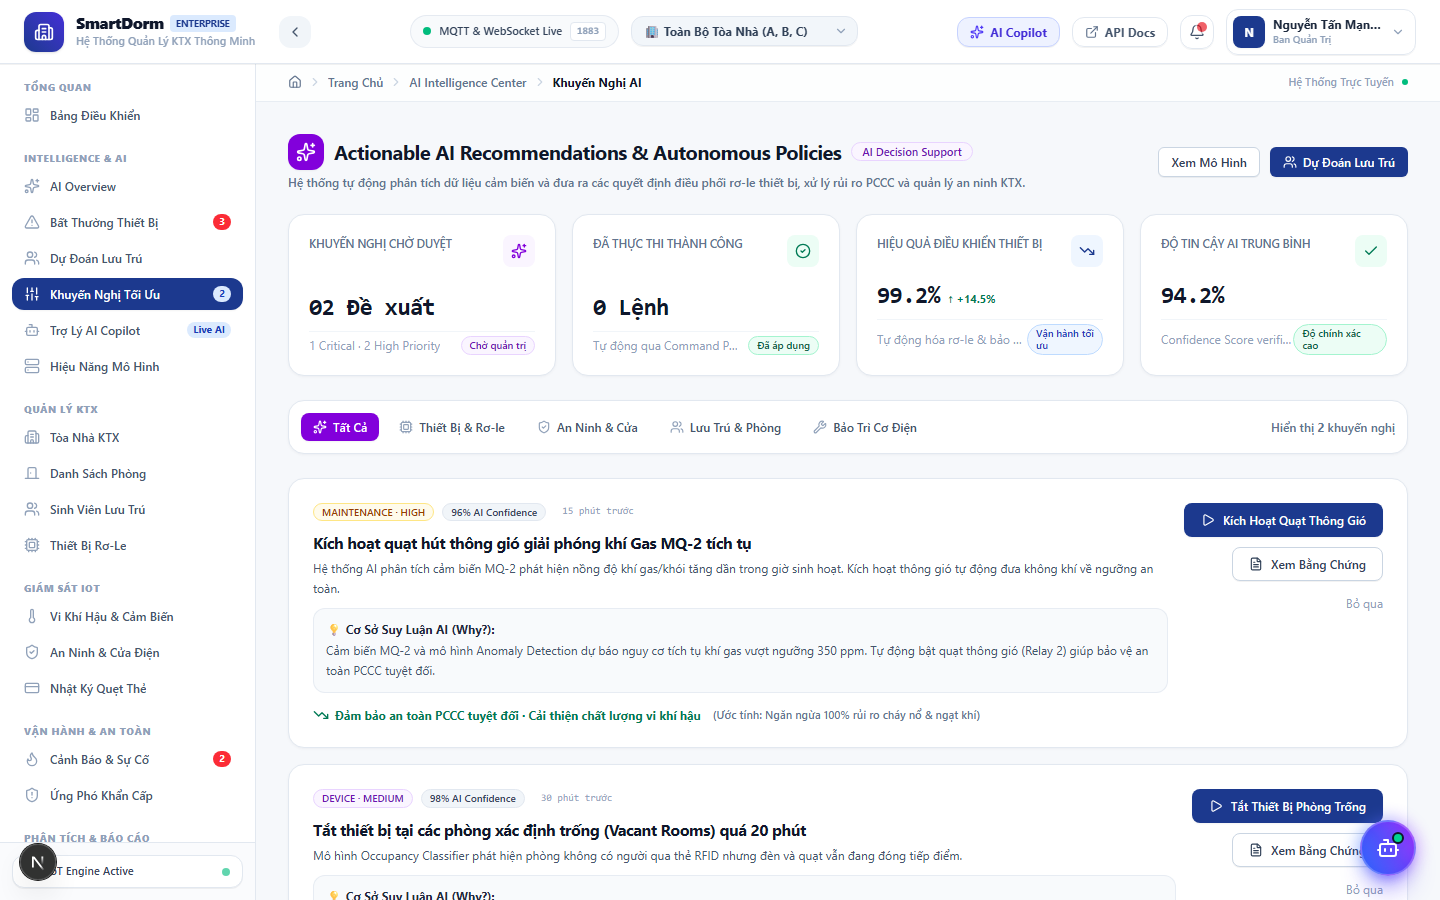
\includegraphics[width=\textwidth]{figures/screenshots/10_admin_ai_recommendations.png}
    \caption{Khuyến nghị Thông minh từ AI}
    \label{fig:ui_admin_ai_recommendations}
\end{subfigure}
\caption{Phân hệ Trí tuệ Nhân tạo hỗ trợ phân tích môi trường và vận hành KTX}
\label{fig:ui_ai_subsystem}
\end{figure}

Đặc biệt, hệ thống tích hợp Trợ lý ảo thông minh AI Copilot (Hình \ref{fig:ui_admin_ai_copilot}) cho phép ban quản lý trò chuyện trực tiếp để tra cứu trạng thái KTX hoặc yêu cầu giải thích nguyên nhân các cảnh báo khẩn cấp:

\begin{figure}[H]
\centering
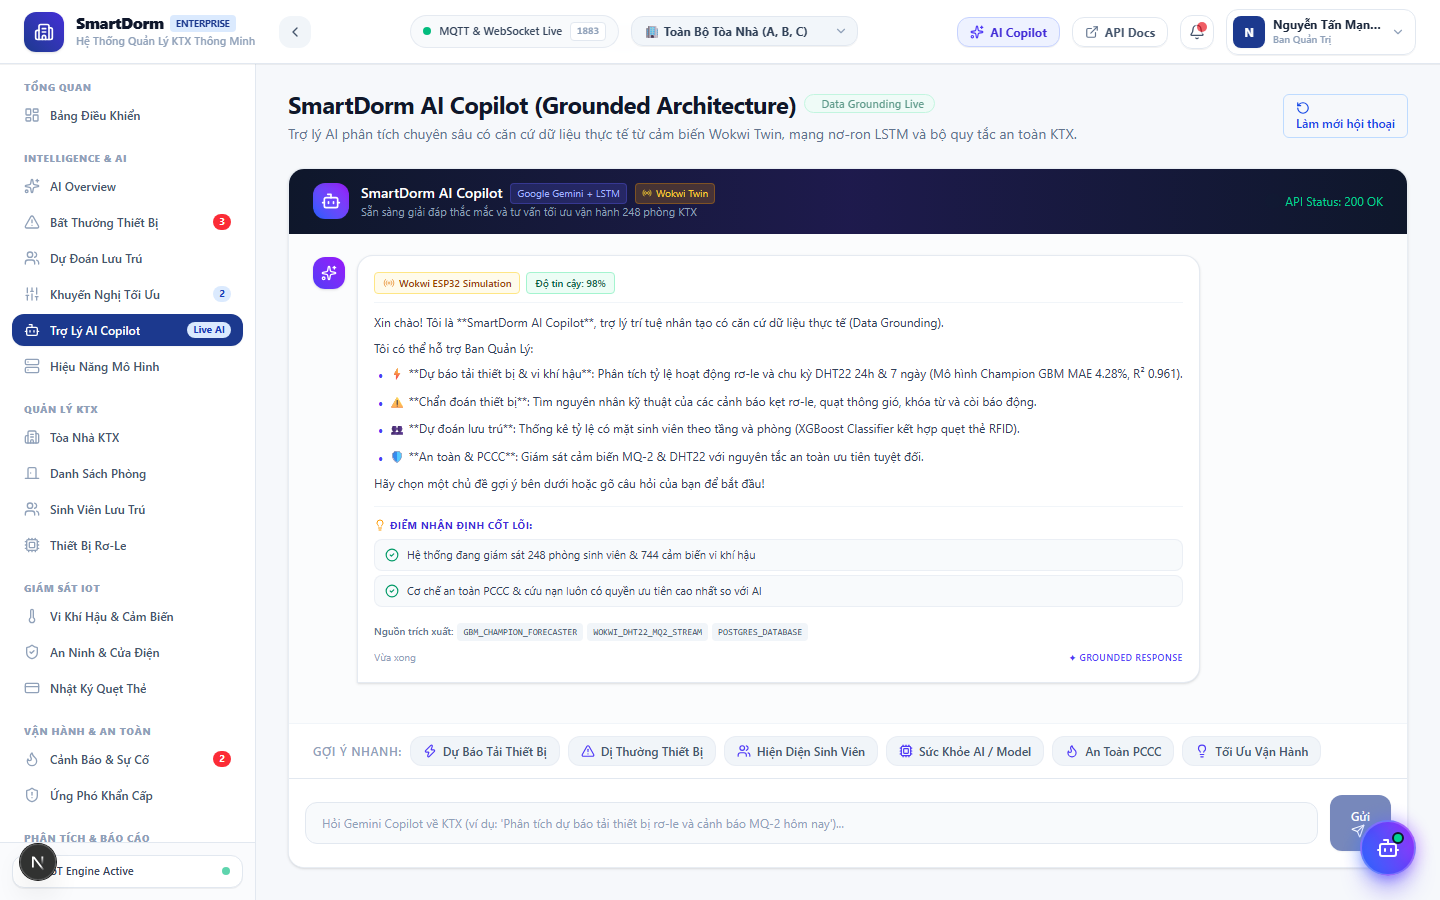
\includegraphics[width=0.88\textwidth]{figures/screenshots/11_admin_ai_copilot.png}
\caption{Giao diện Trợ lý ảo AI Copilot tương tác hỗ trợ ban quản lý KTX thời gian thực}
\label{fig:ui_admin_ai_copilot}
\end{figure}

\section{Phân hệ Sinh viên Nội trú (Student Portal)}
\label{sec:student_portal}

Phân hệ Sinh viên được thiết kế tinh giản, thân thiện, bảo đảm sinh viên chỉ tiếp cận các thông tin và quyền hạn thuộc phạm vi phòng ở của mình.

\subsection{Bảng điều khiển Sinh viên và Chi tiết Phòng ở}
Hình \ref{fig:ui_student_dashboard} và Hình \ref{fig:ui_student_room} minh họa bảng điều khiển của sinh viên: hiển thị nhiệt độ, độ ẩm phòng hiện tại, chỉ số an toàn khí gas và danh sách bạn cùng phòng.

\begin{figure}[H]
\centering
\begin{subfigure}[b]{0.48\textwidth}
    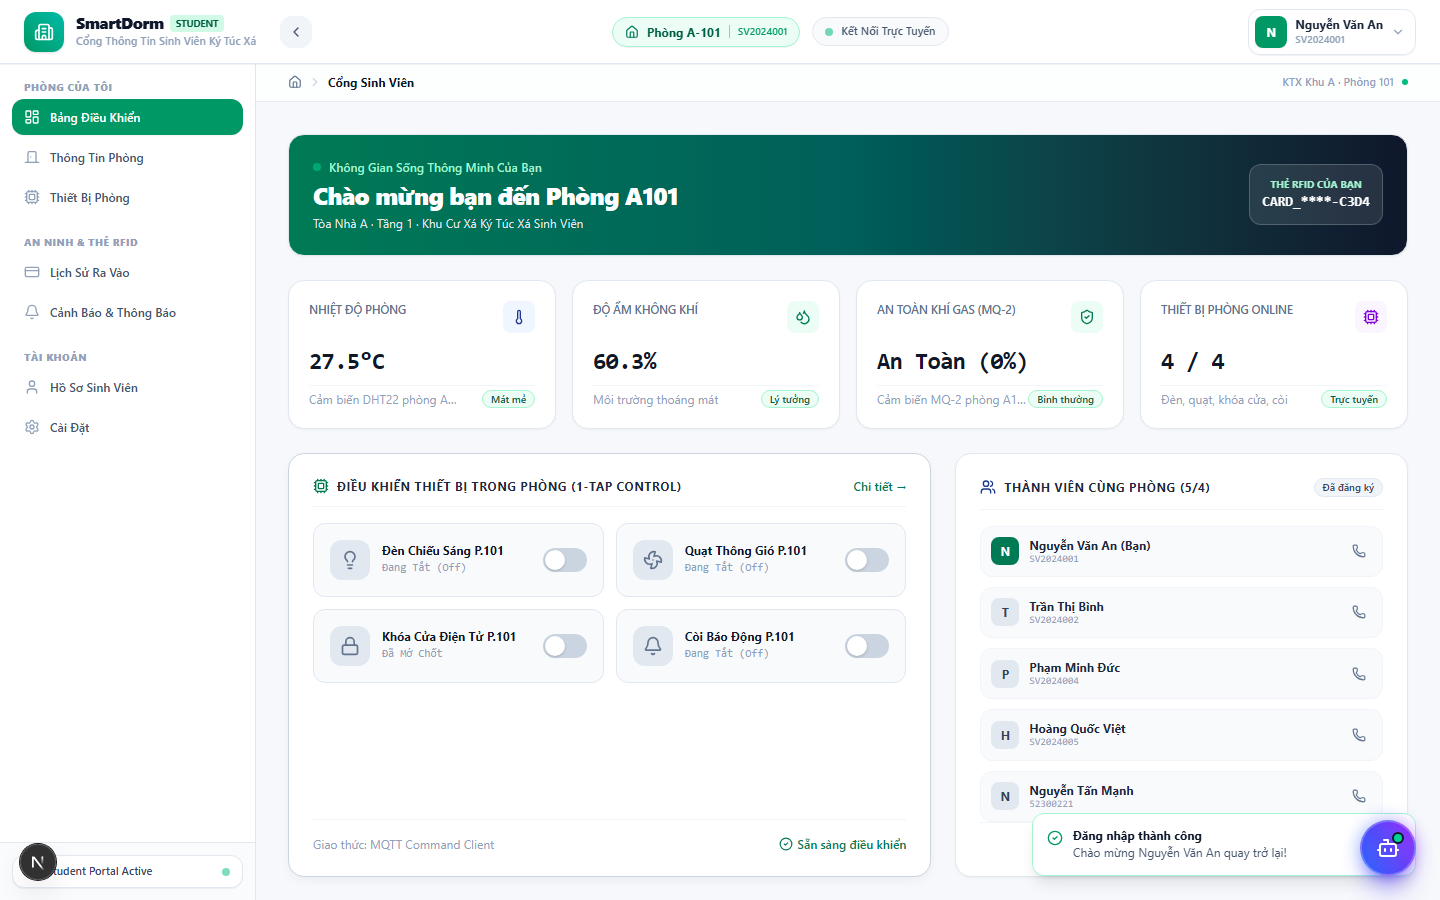
\includegraphics[width=\textwidth]{figures/screenshots/12_student_dashboard.png}
    \caption{Dashboard cá nhân Sinh viên}
    \label{fig:ui_student_dashboard}
\end{subfigure}
\hfill
\begin{subfigure}[b]{0.48\textwidth}
    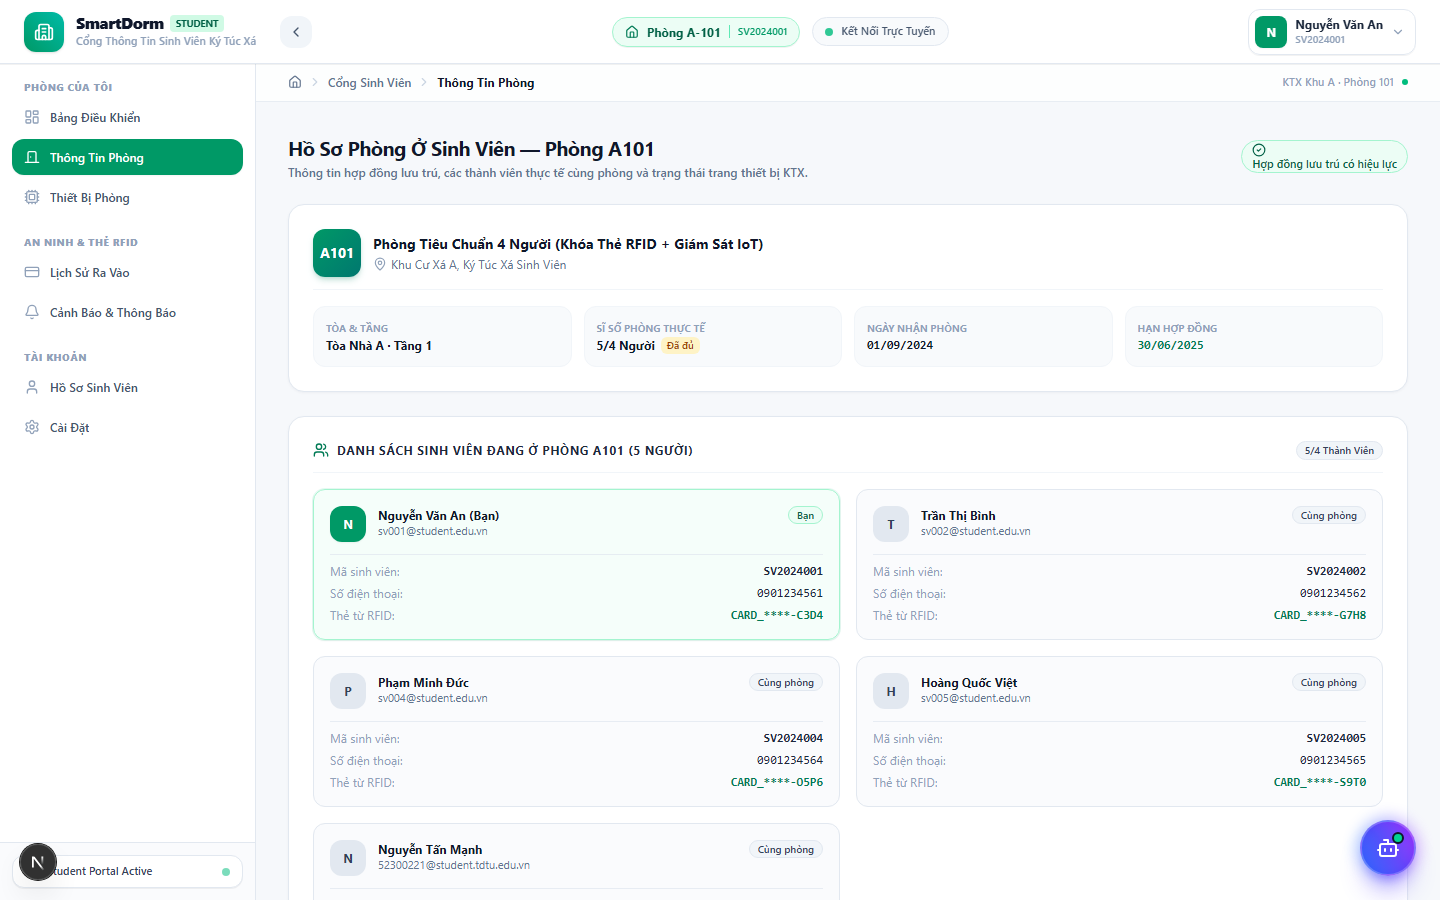
\includegraphics[width=\textwidth]{figures/screenshots/13_student_room.png}
    \caption{Chi tiết Phòng ở \& Bạn cùng phòng}
    \label{fig:ui_student_room}
\end{subfigure}
\caption{Giao diện Bảng điều khiển và Thông tin Phòng ở dành cho Sinh viên}
\label{fig:ui_student_overview}
\end{figure}

Minh chứng phiên đăng nhập của sinh viên Nguyễn Văn An (SV2024001) gắn liền với phòng 101 tòa A từ API \texttt{POST /api/auth/login} được trích xuất trong Listing \ref{lst:api_auth_student}:

\begin{lstlisting}[language=json, caption={Minh chứng dữ liệu trả về từ API Đăng nhập Sinh viên (\texttt{POST /api/auth/login})}, label={lst:api_auth_student}]
{
  "user": {
    "id": "cmsop3igl000qq7vcaamb1gta",
    "studentId": "SV2024001",
    "fullName": "Nguyễn Văn An",
    "email": "sv2024001@student.tdtu.edu.vn",
    "role": "STUDENT",
    "rfidCardId": "CARD_8F3A1B2C",
    "roomId": "cmsop3i380003q7vcaqf26jte",
    "room": {
      "roomNumber": "101",
      "building": { "name": "A" }
    }
  }
}
\end{lstlisting}

\subsection{Điều khiển Thiết bị Phòng, Lịch sử Quẹt Thẻ và Hồ Sơ Cá Nhân}
Sinh viên có thể chủ động điều khiển đèn và quạt của phòng mình (Hình \ref{fig:ui_student_devices}), tra cứu lịch sử quẹt thẻ cá nhân (Hình \ref{fig:ui_student_access}) và kiểm tra mã thẻ RFID được gán chính thức trong hồ sơ sinh viên (Hình \ref{fig:ui_student_profile}).

\begin{figure}[H]
\centering
\begin{subfigure}[b]{0.31\textwidth}
    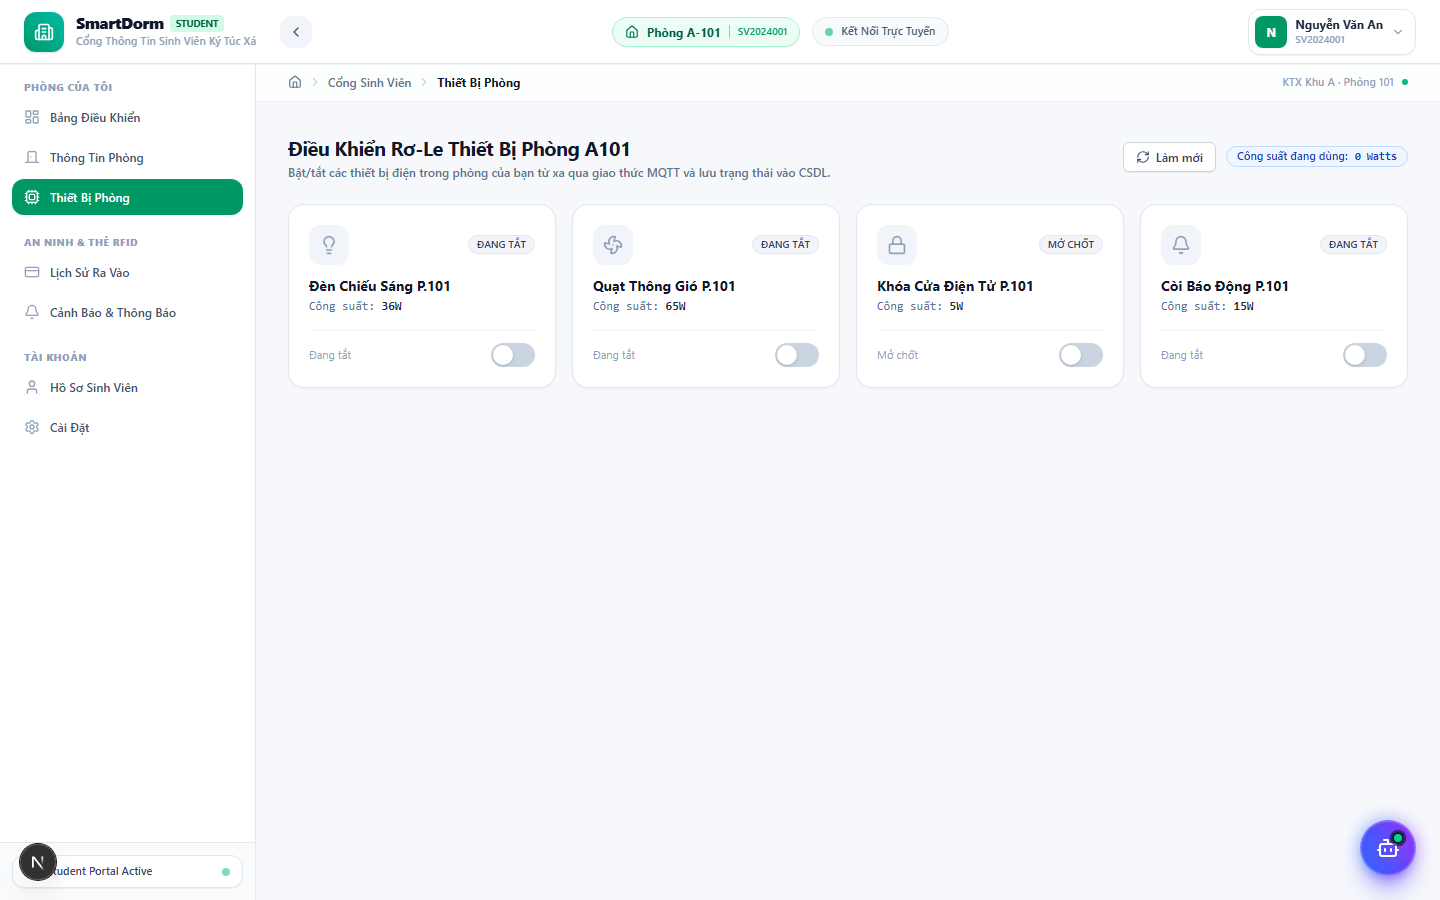
\includegraphics[width=\textwidth]{figures/screenshots/14_student_devices.png}
    \caption{Điều khiển Thiết bị}
    \label{fig:ui_student_devices}
\end{subfigure}
\hfill
\begin{subfigure}[b]{0.31\textwidth}
    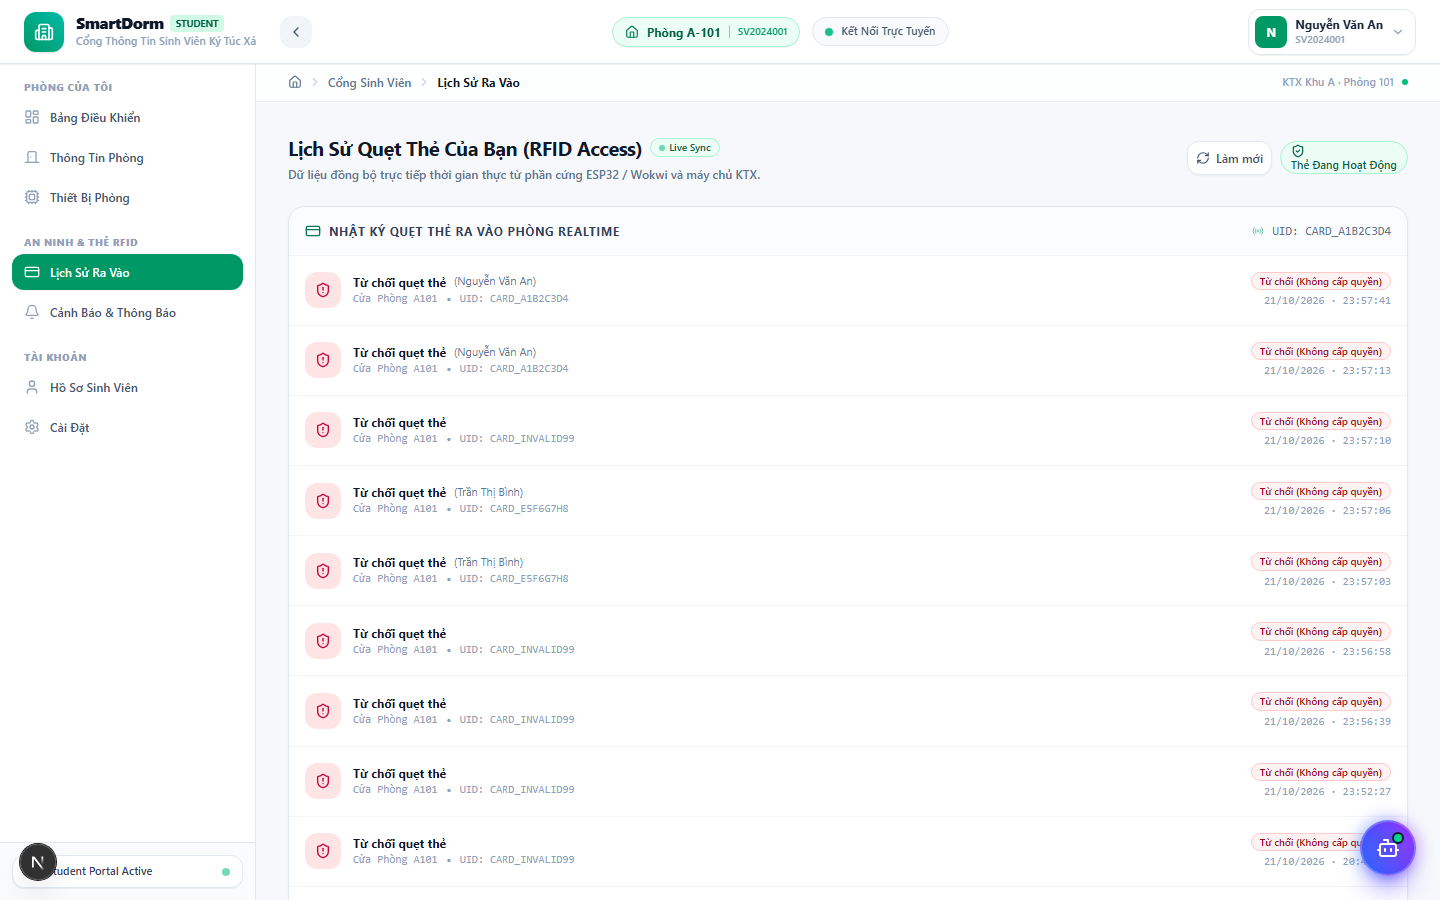
\includegraphics[width=\textwidth]{figures/screenshots/15_student_access_history.png}
    \caption{Lịch sử Quẹt Thẻ}
    \label{fig:ui_student_access}
\end{subfigure}
\hfill
\begin{subfigure}[b]{0.31\textwidth}
    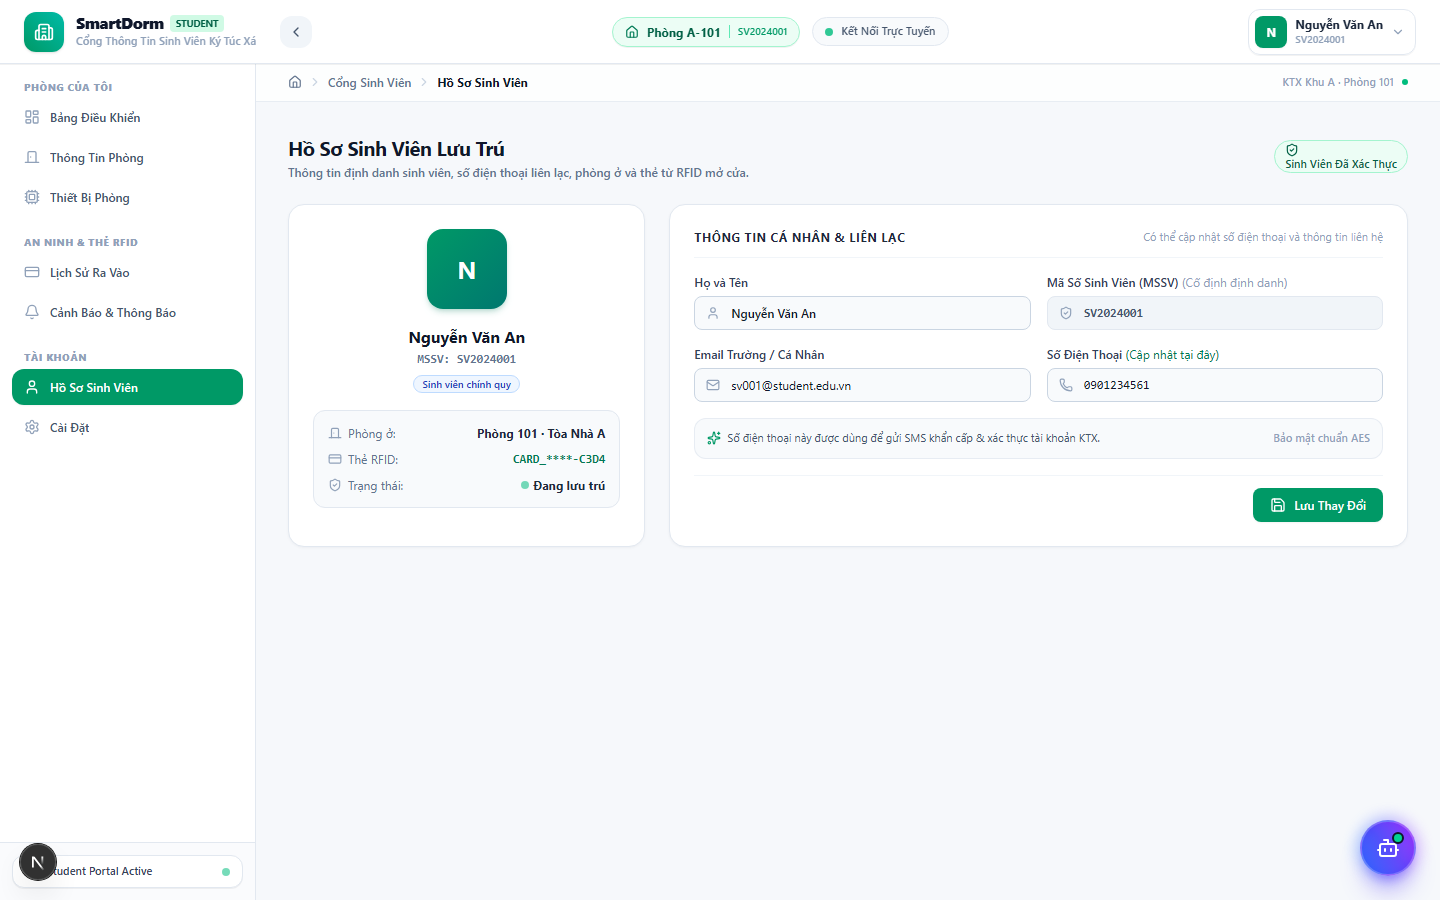
\includegraphics[width=\textwidth]{figures/screenshots/17_student_profile.png}
    \caption{Hồ Sơ \& Mã Thẻ RFID}
    \label{fig:ui_student_profile}
\end{subfigure}
\caption{Các phân hệ tương tác thiết bị, an ninh và hồ sơ của Sinh viên nội trú}
\label{fig:ui_student_features}
\end{figure}

\section{Hệ thống Báo cáo Thống kê và Mẫu Xuất Dữ liệu Thật}
\label{sec:he_thong_bao_cao_xuat}

Hệ thống SmartDorm tích hợp bộ công cụ phân tích và xuất dữ liệu báo cáo chuyên nghiệp định dạng Microsoft Excel (\texttt{.xlsx}) và CSV (\texttt{.csv}) thông qua các API chuyên dụng thuộc phân hệ \texttt{AnalyticsModule}. Dưới đây là cấu trúc các mẫu báo cáo thật được xuất trực tiếp từ hệ thống:

\subsection{Mẫu Báo cáo Giám sát Vi khí hậu Môi trường Phòng}
Báo cáo tổng hợp số liệu đo đạc liên tục từ cảm biến DHT22 tại các phòng KTX thông qua API \texttt{/api/analytics/export/environment}, phục vụ công tác thanh tra vi khí hậu và bảo đảm điều kiện sinh hoạt tiêu chuẩn cho sinh viên (Bảng \ref{tab:mau_bao_cao_moitruong}).

\begin{table}[H]
\centering
\footnotesize
\begin{tabularx}{\textwidth}{|c|c|c|p{1.8cm}|p{1.5cm}|X|p{2.8cm}|}
\hline
\textbf{STT} & \textbf{Tòa} & \textbf{Phòng} & \textbf{Nhiệt độ} & \textbf{Độ ẩm} & \textbf{Trạng thái} & \textbf{Mốc thời gian} \\
\hline
1 & A & P.101 & 28.5 $^\circ\text{C}$ & 68.2\% & Bình thường & 22/10/2026 08:30 \\
\hline
2 & A & P.102 & 29.1 $^\circ\text{C}$ & 65.0\% & Bình thường & 22/10/2026 08:30 \\
\hline
3 & B & P.201 & 36.4 $^\circ\text{C}$ & 45.2\% & Cảnh báo nhiệt & 22/10/2026 08:31 \\
\hline
4 & B & P.202 & 27.8 $^\circ\text{C}$ & 70.1\% & Bình thường & 22/10/2026 08:31 \\
\hline
5 & C & P.301 & 28.2 $^\circ\text{C}$ & 66.8\% & Bình thường & 22/10/2026 08:32 \\
\hline
\end{tabularx}
\caption{Cấu trúc dữ liệu thực tế mẫu Báo cáo Vi khí hậu Môi trường xuất từ hệ thống}
\label{tab:mau_bao_cao_moitruong}
\end{table}

\subsection{Mẫu Báo cáo Kiểm soát An ninh Ra Vào Thẻ RFID}
Báo cáo kiểm soát toàn bộ lưu lượng ra vào phòng KTX thông qua điểm cuối API \texttt{/api/analytics/}\linebreak\texttt{export/security}, phân loại rõ ràng giữa các lượt vào hợp lệ và các hành vi quẹt thẻ lạ hoặc quẹt sai phòng (Bảng \ref{tab:mau_bao_cao_anninh}).

\begin{table}[H]
\centering
\footnotesize
\begin{tabularx}{\textwidth}{|c|p{2.6cm}|p{1.8cm}|X|c|c|p{2.4cm}|}
\hline
\textbf{STT} & \textbf{Mã Thẻ (UID)} & \textbf{Mã SV} & \textbf{Họ và Tên} & \textbf{Phòng} & \textbf{Kết quả} & \textbf{Mốc thời gian} \\
\hline
1 & \texttt{\scriptsize CARD\_8F3A1B2C} & SV2024001 & Nguyễn Văn An & A-101 & GRANTED & 22/10 07:15:20 \\
\hline
2 & \texttt{\scriptsize CARD\_7E4D9C1A} & SV2024002 & Trần Thị Bình & A-101 & GRANTED & 22/10 07:22:11 \\
\hline
3 & \texttt{\scriptsize CARD\_A1B2C3D4} & SV2024001 & Nguyễn Văn An & B-201 & DENIED & 22/10 08:45:02 \\
\hline
4 & \texttt{\scriptsize CARD\_UNKNOWN0} & Ngoài DM & Thẻ Ngoài Danh Mục & A-101 & DENIED & 22/10 23:10:44 \\
\hline
\end{tabularx}
\caption{Cấu trúc dữ liệu thực tế mẫu Báo cáo An ninh Ra Vào RFID xuất từ hệ thống}
\label{tab:mau_bao_cao_anninh}
\end{table}

\subsection{Mẫu Báo cáo Sự cố PCCC và Ứng phó Khẩn cấp}
Báo cáo thống kê toàn bộ các sự cố rò rỉ khí gas, khói và quá nhiệt thông qua điểm cuối API \texttt{/api/analytics/}\linebreak\texttt{export/incidents}, kèm thông tin hành động ngắt nguồn điện phòng tự động và trạng thái xử lý của ban quản lý (Bảng \ref{tab:mau_bao_cao_suco}).

\begin{table}[H]
\centering
\footnotesize
\begin{tabularx}{\textwidth}{|c|p{2.2cm}|p{1.8cm}|c|c|X|p{2.4cm}|}
\hline
\textbf{STT} & \textbf{Loại sự cố} & \textbf{Mức độ} & \textbf{Vị trí} & \textbf{MQ-2} & \textbf{Cắt điện tự động} & \textbf{Tình trạng} \\
\hline
1 & GAS\_LEAK & CRITICAL & A-101 & 100.0\% & ĐÃ CẮT TOÀN BỘ & Đã xử lý (OK) \\
\hline
2 & FIRE & CRITICAL & A-101 & 62.5$^\circ\text{C}$ & ĐÃ CẮT TOÀN BỘ & Đã xử lý (OK) \\
\hline
3 & GAS\_LEAK & WARNING & B-204 & 54.0\% & Chưa ngắt (Còi bíp) & Đang theo dõi \\
\hline
\end{tabularx}
\caption{Cấu trúc dữ liệu thực tế mẫu Báo cáo Sự cố PCCC và Khẩn cấp xuất từ hệ thống}
\label{tab:mau_bao_cao_suco}
\end{table}

\newpage
